% Template for ICIP-2019 paper; to be used with:
%          spconf.sty  - ICASSP/ICIP LaTeX style file, and
%          IEEEbib.bst - IEEE bibliography style file.
% --------------------------------------------------------------------------
% \documentclass{article}
\documentclass[xelatex,ja=standard]{bxjsarticle}
\usepackage{spconf,amsmath,graphicx}
\usepackage{amsmath}
\usepackage{algorithm}
\usepackage[noend]{algpseudocode}

% japanese packages
\usepackage{xeCJK}

\usepackage{tikz}

\makeatletter
\def\BState{\State\hskip-\ALG@thistlm}
\makeatother

\usepackage{multicol}
\usepackage{multirow}

% Example definitions.
% --------------------
\def\x{{\mathbf x}}
\def\L{{\cal L}}

% Title.
% ------
\title{An Occlusion Diminishing Robot Vision System with Mirror Reflections}
% Occlusion Reducing Robot Vision System utilizing Mirror Reflections


% Single address.
% ---------------
\name{Kentaro Yoshioka, Hidenori Okuni, Tuan Thanh Ta, Akihide Sai}
\address{Toshiba Corp.}
%
% For example:
% ------------
%\address{School\\
%	Department\\
%	Address}
%
% Two addresses (uncomment and modify for two-address case).
% ----------------------------------------------------------
%\twoauthors
%  {A. Author-one, B. Author-two\sthanks{Thanks to XYZ agency for funding.}}
%	{School A-B\\
%	Department A-B\\
%	Address A-B}
%  {C. Author-three, D. Author-four\sthanks{The fourth author performed the work
%	while at ...}}
%	{School C-D\\
%	Department C-D\\
%	Address C-D}
%
\begin{document}
\ninept
%
\maketitle
%
\begin{abstract}
Blind spots are one of the biggest issues in robot vision for manipulation, and if the target object is hidden in the blind spot, the object recognition and gripping accuracy will be reduced. In the worst case, the target may be dropped on the way or hit around and damaged. I will. For example, if a large number of robot arms cooperate in a single workplace, blind spots will be created at the robot's hand using only the zenith sensor, and this will be a severe environment for robot vision. The blind spot can be greatly reduced by increasing the number of installed distance sensors, but the increase in sensor cost cannot be ignored, and if the robot arrangement changes, the sensors need to be rearranged.
In order to solve the problem of blind spot, we propose a robot vision system that reduces blind spot using mirror reflection without increasing the number of sensors. The blind spot is greatly reduced by reflecting light rays with a mirror and sensing a non-linear field of view from a zenith sensor. Since the proposed mirror reflection system detects the blind spot existing on the workplace and performs reflection sensing to remove it, even if the robot arrangement changes, sensor rearrangement is not required and the blind spot can be effectively removed. The only elements to be added to the system are a commercially available mirror and a tilt-to-pan unit, and the cost is lower than adding a sensor.
Through experiments, it is shown that the proposed mirror reflection sensing can obtain almost the same point cloud data and object detection accuracy as when multiple sensors are installed when sensing environments with many blind spots. (A little more?)

マニプレーション用のロボットビジョンにおいて死角は最大の課題の1つであり、死角でターゲット物体が隠れると物体認識や把持精度が下がってしまい最悪の場合ターゲットを途中で落としたり周辺にぶつけ破損させてしまう。例えば多数のロボットアームが1つの作業場で協働すると天頂センサだけではロボット手元に死角が生じるため、ロボットビジョンにとって厳しい環境となる。設置する距離センサの数を増やすことで死角を大きく減らす事は可能だが、センサコストの増加は無視できず、またロボット配置が変わるとセンサの再配置が必要である。
そこで我々は死角の課題を解決するため、センサを増やさずミラー反射を用いて死角を低減するロボットビジョンシステムを提案する。ミラーで光線を反射させ天頂センサから非直線上の視野をセンシングすることで死角を大幅に低減する。提案するミラー反射システムは作業場上に存在する死角を検出しそこを取り除くよう反射センシングを行うため、ロボット配置が変わってもセンサ再配置は必要なく効果的に死角を除去可能である。システムに追加する要素は市販ミラーとチルトーパンユニットのみであり、センサを追加するのに比べコストは低い。
実験を通じ、提案するミラー反射センシングは死角の多い環境をセンシングした場合複数センサ設置時とほぼ同等の点群データおよび物体検出精度が得られる事を示す。(もう少し?)
\end{abstract}
%
\begin{keywords}
One, two, three, four, five
\end{keywords}
%

%%%%%%%%%%%%%%%%%%%%%%%%%%%%%%%%%%%%%%%%%%%%%%%%%%%%%%%%%%%%%%%%%%%%%%%%%%%%%%%%%
\section{Introduction}
ロボットマニプレーションシステムは生産性向上や省人化の実現を図ることができるため製造現場や運送業界で導入が急速に進んでいる。このようなシステムのロボットビジョンはセンサで取得した周囲情報から物体の位置や形状を認識しロボットの作業を決定する。そのためターゲット物体がセンサの死角となると物体が存在しないと誤認したり間違った姿勢を推定してしまい、ロボットは正常に作業を完遂できないばかりか把持を失敗しターゲット物体を途中で落としたり周辺にぶつけ破損させてしまう。このようにロボットビジョンシステムでは死角が最大の課題の一つである。

そこでロボットビジョンでは死角を出来るだけ減らす試みがなされてきた。例えばロボット天頂にセンサを取り付けるのは最も死角が少ないためで、商業ロボットの多くはそのような構成をとっている\cite{mujin}\cite{toshiba}\cite{righthand}。
しかしながらロボットアームが作業スペースで動くと、アーム直下には必ず死角が生まれる。このようなロボット自身または他の作業ロボットが物体上空で動作することで作り出す死角を本論文ではブロッカー死角と定義する。ブロッカー死角が発生すると物体が欠けてしまうため認識が難しくなるだけではなく、最悪完全に物体が隠れてしまい見落としてしまう。ロボットが単体であればアームが作業場所から退いた後にセンシングすることでブロッカー死角を防ぐことはできるが、ロボットの作業速度は落ちてしまう。さらにはロボット自動化システムの将来の形の1つは、人も含め複数のロボットが協調して1つまた複数の作業をこなす形態である。この場合複数のロボットが作業空間上で絶え間なく動作するため天頂のセンサからの死角は多く、各ロボットが高い認識精度を達成するにはさらにブロッカー死角の少ないロボットビジョンシステムを構築する必要がある。

またロボットビジョンには根本的な死角があり、センサの視線上にない物体面は捉えることができず、例えばセンサ真下にある物体の側面はセンシングできない。このようなセンサの死角を本論文では側面死角と定義する。ロボットが把持する際には物体のCADデータといったOracleとセンシング結果をマッチングし姿勢推定を行う。そのためセンシング結果から物体の側面情報が欠けてしまうと姿勢推定精度は律速され把持の成功率も低下してしまう可能性がある。

従来の課題に対するアプローチ
ブロッカーと側面の両死角を減らす最も有効な手法はシンプルにセンサ数を増やし、複数アングルからセンシングすることである。一方でこの手法はセンサコストが跳ね上がってしまう。2Dカメラに比べると高精度距離センサ\cite{velodyne}\cite{ensenso}の価格は高く、ロボットシステムの総コストを削減するためには使用する距離センサ数は最低限であることが望ましい。また協同ロボットの配置方法により最も死角を減らせる最適センサ配置は異なる。そのためロボットの配置や作業内容に応じ随時センサ配置も変える必要があり、複雑な作業を行う協同ロボットシステムに適応するには柔軟性が欠ける。
また距離センサをロボットアームのエンドエフェクタにつけ、対象物を複数角度からセンシングするようにアームを動作させることでセンサ1つでも死角を大きく減らせる\cite{Schwarz2017}。しかしながら産業用ロボットは作業スループットを最大化するのが大きなクライテリアである。死角を取り除くため、ターゲット上で複数回場所を変えながらセンシングすると本来の作業時間を圧迫してしまいロボット作業効率が低下する。また文献\cite{Holz2015}ではセンシング時間を減らすため、アームセンサと天頂センサの2つでシステムを構築している。この構成では動作時間を短縮可能だが距離センサ数は倍になりコストは増加してしまう。

まとめると従来から死角低減に挑戦したシステムは多いが、いずれのアプローチも作業効率低減かセンサコスト増どちらかのトレードオフが生じていた。

本研究について
我々は世界で初めてミラー反射センシングを用いて死角を低減するロボットビジョンシステムを提案する。ロボット周辺に取り付けた市販ミラーで光線を反射させ非直線上の視野をセンシングすることで死角を大幅に低減する。さらに本システムは適応的に作業場上に存在する障害物を検出し、生じたブロッカー死角を除去するようにミラー反射センシングを行う。そのためセンサ数は1つと低コストな実装にも関わらず、あたかも複数センサを最適配置した場合に近い結果を得る。
ミラーを利用し非直線上の死角をセンシング出来ることは従来から知られてきたが、ロボットビジョンシステムの性能を向上するためミラー反射を応用した研究はなかった。今回のシステムで追加するハードウェアはパン制御可能な雲台と市販されているミラーのみでセンサを追加するのに比べコストは大幅に削減できる。
またミラーのズレに対する自動キャリブレーションを提案する。長期間稼働によってミラーの設置角度や位置がズレてしまうとセンシング誤差につながる。そこでロボット自身をマーカーとする自動キャリブレーションを提案。ミラーキャリブレーションに適したロボット姿勢を探索することで、実験を通じミラーが+- XX度動いても自動キャリブレーションによりセンシング誤差をX cm以内に抑えた。
そして我々は実験を通じミラー反射センシングはセンサ数を増やす事と同等の効果がある事を確認した。ブロッカー死角低減の効果を実証するため、ダンボール上をロボットアームがランダムに動作するデータセットで物体検出精度を評価。直接センシングのみでは死角が多く認識精度は低いところ、直接と反射センシングを結合することでmAP精度はXX\%向上することを確認し、これはセンサ2つを用いた精度とほぼ同等であった。


%%%%%%%%%%%%%%%%%%%%%%%%%%%%%%%%%%%%%%%%%%%%%%%%%%%%%%%%%%%%%%%%%%%%%%%%%%%%%%
\section{Related researches}
\textbf{ミラーやミラー反射点群の検出}
Laser range finder(LRF)やLiDARといったセンサにおいて環境に存在するミラーやガラスでレーザが意図せぬ反射をしてセンシングに誤差が生じてしまうのが課題であった。センサにはレーザがミラーで反射したと認識できず、反射が生じるとミラーの奥に物体が存在するかのような"虚像"を観測してしまう。SLAMやマッピング等のタスクにおいて虚像は悪影響を与えるため、虚像を取り除くまたは実像に変換する研究が行われてきた\cite{Yang2008}\cite{Yang2011}\cite{Kim2016}\cite{Yun2018}\cite{Kashammer2015}。一般的には空間に存在する実像とミラー反射の虚像間で相関マッチングを取ることで虚像を検出・除去するというアプローチを取る。

また移動中のロボットにとって鏡は障害物であるため、ロボットが避けるためには鏡の存在自体を検出する必要がある。鏡はレーザ光を反射しカメラでも反射像を写してしまうため、鏡の検出は難しい研究タスクである\cite{Whelan2018}。LRFとカメラを組み合わせたフュージョンアプローチ\cite{Yang2008}やカメラ画像からディープラーニング技術を用いて検出する手法\cite{Yang2019}が提案されている。一方で我々のシステムでは恣意的にミラーをロボット動作環境に配置するため大まかなミラー位置は既知であり、改めて検出する必要はない。

\textbf{ミラー反射を用いたロボットビジョンシステムの性能向上}
環境に置かれたミラーの反射影響を取り除く研究は多いものの、恣意的にミラーを配置し反射を有用に使いロボットビジョンシステムの向上を狙った研究は多くない。数少ない先行研究のRef.\cite{kulpate2005eye} \cite{Marchand2017}はミラーを使うことでカメラFoVを超えた位置からのロボットのビジュアルサーボを実現する。またSaccade mirror\cite{okumura20151}はミラーと高速パン/チルト機能で広いFoVを持つ高速ビジョンシステムを実現しRef.\cite{Noguchi2012}はLiDARの脇にミラーをつけることでセンサのFoV拡充を狙う。
いずれの研究もカメラのFoVを拡充するシステムであり、我々の目的であるロボットビジョンシステムのブロッカー死角低減とは異なる。


\section{ミラー反射センシング 1.5-2ページ}

%%%%%%
\begin{figure}[!]
\centering
  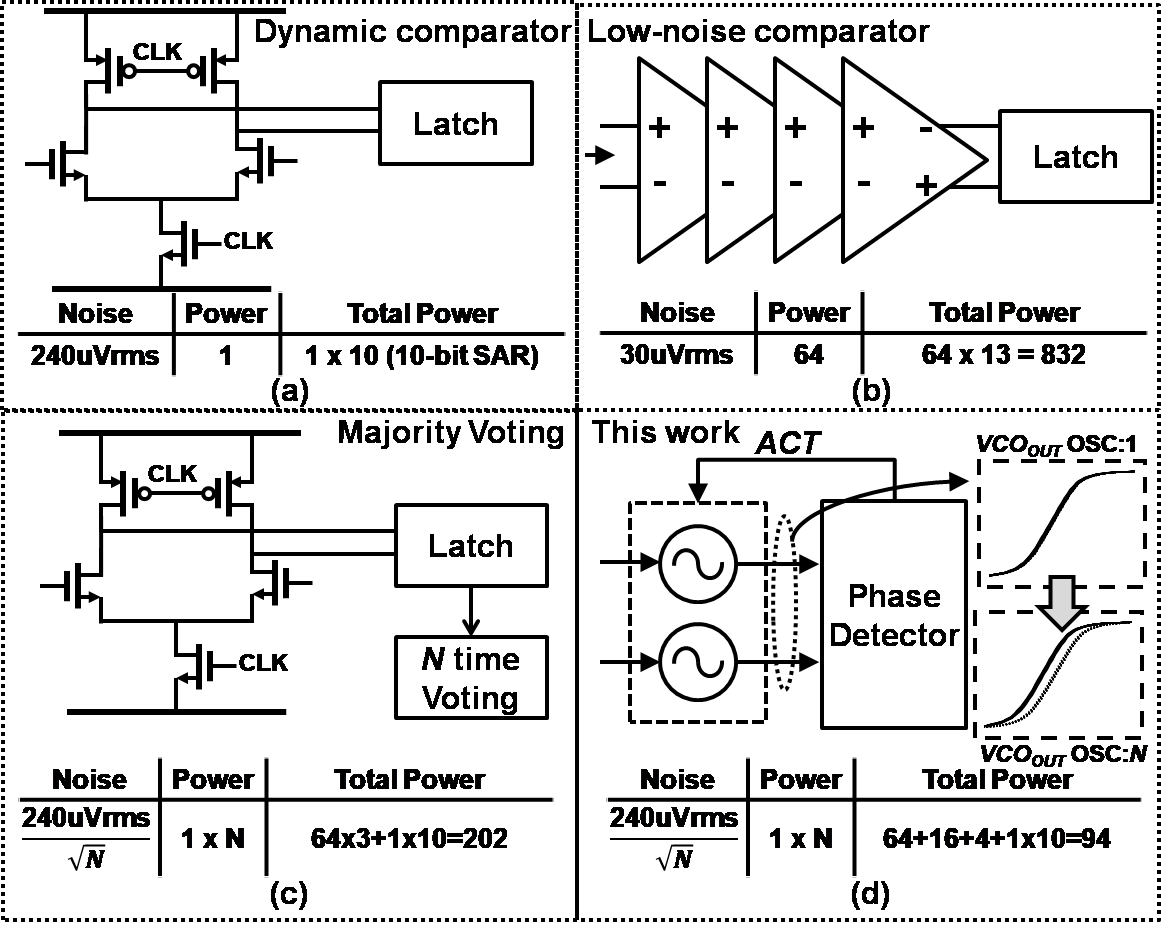
\includegraphics[width=0.5\textwidth]{figure/fig1.png}
  \caption{caption..}
  \label{fig-concept}
\end{figure}
%%%%%%%

\subsection{ミラー反射センシングシステムについて}
天頂につけた距離センサによりロボットの作業スペースをイメージングするロボットビジョンシステムは産業用のビンピッキングやマニプレーションロボットにおいて多く見られる構成である。だがこのようなシステムでは天頂センサから死角になる箇所はセンシング出来ない。具体的にロボットマニプレーションで課題となるのは第1にブロッカー死角である。これはロボットアーム自身または他作業ロボットが作業空間上に覆いかぶさってしまう事で作成してしまう死角である。もし複数台のアームが作業していると耐えず天頂センサから死角を作成してしまい、物体の誤検出や見落としが増加してしまう。図1の上部の写真ではロボットアームが作業空間上のトマトに覆いかぶさり生じたブロッカー死角を例として示している。天頂につけられたセンサからはアーム直下のトマトは完全に死角となってしまうため、得られた点群データからは完全にトマトが欠けてしまう。

第2に課題となるのは側面死角である。例えばセンサ直下の物体の側面といったセンサの直線状にない箇所は死角となってしまう。例えば図1の上部ではピーマンの上部をセンシングできているが、側面の点群は欠ける。このような物体のカバレッジ不足は把持に必要な物体姿勢推定の精度を低下させてしまう。

我々はブロッカーと側面死角をミラー反射センシングによって死角を低減するロボットビジョンシステムを提案する。提案するビジョンシステムのコンセプトを図1に示す。本論文では従来と同等に作業スペースを直接センシングする事を"Direct Sensing(直接センシング)"と呼称し、ロボットの作業空間側面に取り付けたミラーに反射させセンシングする事を"Reflection sensing(反射センシング)"と呼称する。我々はこの2つのセンシングを組み合わせることで、死角の少ないセンシング結果を得る事を狙う。ミラーを介して光線を反射させることで”non-line-of-sensing(非直線センシング)”が可能となり、あたかももう1つセンサをミラー箇所に取り付けたかのようなセンシング結果を得られる。例えば図1中部に示す通り、センサをチルトさせ作業空間側面のミラーに反射させセンシングを実施する事でロボットアーム真下にあったトマトをセンシングすることが可能となる。また天頂からではなく側面からセンシングしているため、トマトの側面情報も取得しておりブロッカー死角と側面死角の両者を低減可能であることがわかる。

一方で反射センシング単体のみでは十分に死角を減らすことは出来ない。図1中部に示すとおり反射センシングを行ってもロボットアームによるブロッカー死角は生じてしまい、図中ではピーマンがブロッカー死角により欠けてしまう。死角を効率よく減らすには直接センシング、反射センシングの両方を実施しその結果を足し合わせることである。図1下部に示すとおり2つのセンシング結果を足し合わせることで作業空間にあったトマトとピーマン2つの物体を含んだデータが得られる。
(簡単のため説明はセンサとミラーは1つずつであると記述する。本フレームワークにおいてミラーの数は拡張可能、更に死角をへらすことができる。センシング時間とトレードオフ。実験結果では更に増やしたときの結果を提供する。)


\subsection{信号処理パイプラインについて}
%%%%%%
\begin{figure*}[ht!]
\centering
  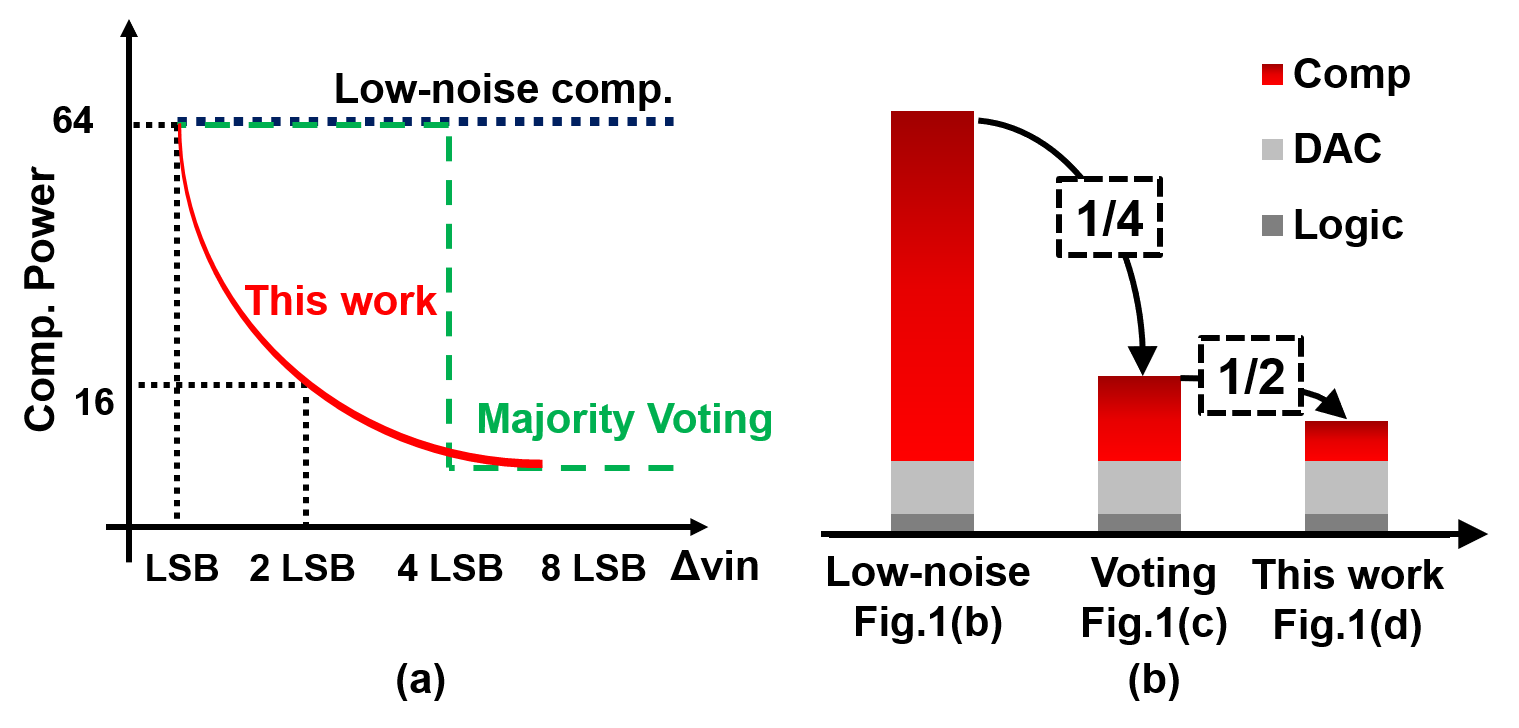
\includegraphics[width=0.75\textwidth]{figure/fig2.png}
  \caption{caption..}
  \label{fig-concept}
\end{figure*}
%%%%%%%
本システムの信号処理パイプラインを図 2に示す。
信号処理の狙いは直接センシング結果からブロッカー死角を検出し、その検出されたブロッカー死角を最も減少させるように反射センシングのスキャン角度を決定する。
図2を元に大まかな流れを説明する。まず直接センシングを行い作業空間のデータを得る。その結果からブロッカー死角の検出を行い、ブロッカー死角を中心にセンシングするようにミラー反射におけるスキャン角度(チルトユニットの回転角度)を決定する。そして反射センシングを実施しブロッカー死角の少ないセンシング結果を得る。得られたセンシングデータはミラー座標であるため、世界座標に変換することで直接センシング結果と結合できるようになる。直接と反射センシング結果をあわせた結果を元に物体検出や姿勢推定といった検出タスクを実施する。以後のセクションでは各ブロックに関して詳細を説明する。

	ブロッカー死角の検出について
作業領域上空で動作するロボットアームや協働作業する人間等がブロッカー死角を作り出す。このようなブロッカー死角の検出アプローチはいくつか方法がある。

今回の実装では単純だが効果的なルールベースアプローチでブロッカー死角を検出する。作業空間上に存在しうる物体の最大高さを定義し、その高さを超える物体が検出された場合はブロッカーとして検出する。高さしきい値を超えた範囲の面積を導出し、ある面積以上のブロッカーが存在する場合そのエリアをブロッカー死角と判定する。面積でもフィルタリングすることでセンサノイズの影響を排除することができる。この手法は単純であるものの、一般的にロボットアームは周囲物体を避けて物体をマニプレーションするためある程度の高さにアームを配置するため、このような単純なルールベースでも上手くブロッカー死角を検出できる。
この時生じた最も大きいブロッカー死角エリアの重心を検出結果として出力し、本座標を元に反射センシングのスキャン角度を設定する。

また画像認識を用いてブロッカー物体を検出するアプローチを使用しても良い。
学習にデータが必要でDNNを使用するとレイテンシが長いといった欠点はあるが、ルールベースではカバーできないレアケースもカバーできる。(ロボットアームが低い高さから侵入した場合や小さい物体をマニプレーションする場合など)

	スキャン角度の決め方について
原理
カメラ位置とスキャン座標(例えばブロッカー死角の中心)の2点を定めれば一意に角度は決まる。
ミラーに対してスキャン座標の虚像点を作ってやり、そこを結んだ線の角度がスキャン角度となる。

実際のアプローチ
ミラー→世界座標の回転行列がキャリブレーションで求められている。その逆行列をかける事でスキャン座標をミラー座標系で示した座標が求まる。
虚像スキャン点とカメラ位置を結ぶ線からスキャン角度を導出可能。
ミラーに角度がついていてもちゃんと動く。


有用なデータを得るために、興味のある領域をセンシングするようにスキャン角度を設定する必要がある。ここでは図 1におけるセンサスキャン角度変更機構におけるスキャン角度決定方法の実施例について述べる。

 
図 3 直接センシング時の座標関係

直接センシング時に最適なスキャン角度θを決定するには2つの座標がわかれば良い:
・センサの設置位置
・センシングしたいスキャン空間の中心点(ターゲット座標)

ここでは図 5のように単純のため二次元空間で議論をする。
センサ設置位置を[xs,ys]、ターゲット座標を[xt, yt]とした場合、目標とするスキャン角度θは
θ=arctan⁡((yt-ys)/(xt-xs))
と一意に求めることができる。

 
図 4 反射面がある場合のスキャン角度決定方法

またミラー反射を用いる時の最適なスキャン角度θを決定するには3つの座標がわかれば良い:
・センサの設置位置
・反射面の存在する領域
・センシングしたいスキャン空間の中心点

ここでは必ず反射面を通り、スキャン空間の中心点を経由するようなスキャン角度θを求める。また単純のため反射面はy軸と平行の領域であると考える(反射面はx=xmと表現)。
するとターゲット座標を反射面に線対称の点にvirtual targetとして虚像を作成し、その点とセンサ座標を結んだ直線をセンサとターゲットを結ぶ線として考えられる(図 6)。この時虚像ターゲットの座標は[xt+2*xm, yt]として表される。
2点を結ぶ直線が得られたため、スキャン角度は先程と同様に:
θ=arctan⁡((yt-ys)/(xt+2*xm-xs))
と一意に求めることが可能である。

このように図 1のセンサスキャン角度変更機構に必要なセンシング座標とミラー反射の有無を入力することで、所望のスキャン角度を導出し距離センサのスキャン角度を制御してもよい。

	ミラー反射の処理
ここでは反射が起きた時のセンサデータを直接センシングデータと同時に活用するため、虚像を実像に復元する過程についての実施例を述べる。
以降では距離センサを基準とする座標系を世界座標、ミラー反射した座標系をミラー座標と呼称する。
物体検出やロボット動作は世界座標基準で行うため、ミラー座標を世界座標に変換する処理が必要である。

原理
ミラーは軸上の反転。ミラー位置座標に平行移動の後にx軸上で反転。そしてまた世界座標に戻せば良い。
これを丁寧に書き下すと行列の合成として書くことができる。

実際のアプローチ
上記の原理から、カメラからミラーの距離と傾き角度を測定することでミラー座標→世界座標。
より一般的なアプローチは4x4行列をキャリブレーションなどで取得し、一度に計算すること。

距離センサは反射面(ミラー)越しにデータを取得したとしても、鏡における反射が起きたという情報は織り込まない。そのため図 4のように鏡の向こうにターゲット物体が存在するようにデータを出力する。本稿ではこのように距離センサが誤認した鏡越しの物体を虚像と定義する。
鏡像データを有効活用するためには虚像を正しい座標情報に復元する必要があり、ここではその信号処理の実施例について述べる。このような信号処理を図 1のセンシング結果処理機構内で行い、出力する3次元センシング情報から虚像を修正し正しい座標情報に変換しても良い。

一般的には虚像を復元するためには反射面に対して線対称の座標を求めてやればよい。そのためにはターゲット虚像を反射面がx軸と重なり合うような座標空間に変換する必要がある。このような座標空間に変換する4行4列の変換行列をHmirrorとする。そしてx軸上で反転するような変換行列Hflipをかけ合わせればよい。このような4行4列の変換行列Hflipは以下のように表される。
Hflip= [■(-1&0&0&0@0&1&0&0@0&0&1&0@0&0&0&1)]
その後に元の座標空間に戻してやれば良い。その時はHmirrorの逆行列、Hmirror-1を掛ければ良い。上記をまとめると正しい座標情報にセンサデータが取得した虚像を変換するには、
%target=H_mirror H_flip H_mirror^(-1) [■(xi&yi&zi&1)].T
といった行列演算を行えば良い。例えばシステム立ち上げ時にHmirrorを導出すれば、動作中には予め求めたHmirrorを使用し虚像補正を実施すれば良い。また反射面が複数ある場合にはHmirror行列は反射面に応じて異なるため、反射面毎にHmirror行列を求める必要がある。


\section{キャリブレーション (1ページ)}
上記信号処理パイプラインにより、ミラー座標から世界座標に変換する行列式を知ることがミラー反射ビジョンシステムを構築する上で必須。
一方で工場などの振動の多い箇所に設置しているとフレームのたわみやズレなどによってミラー位置がズレたり角度が変わってしまう。

例えばミラー角度が5度キャリブレーション時からズレてしまうと、虚像復元時に正解データとxx cmも点群データがズレてしまう。(図を出す)
このようなデータでは正常な物体認識をすることはできず、反射データは役に立たない。

このようにミラー反射ビジョンシステムの実用化を考える上でミラー座標の自動キャリブレーション機能は必須である。
キャリブレーションはキャリブレーションプレートなどの基準物があれば容易に実施することができる。
しかし装置稼働中にキャリブレーションプレートを配置するのはダウンタイムを増加してしまうため現実的ではない。
またロボットが作用する対象物も設置環境によって変わってしまうため、良いキャリブレーションターゲットではない。
ミラー反射すると対象物は左右反転するが、左右対称なキャリブレーションターゲットでは反射時と非反射時の点群、
どちらでもキャリブレーションが収束してしまうため望ましくない。

我々はロボット自身をキャリブレーションターゲットとしてミラー座標の自動キャリブレーションを行う事を提案する。
ロボットアーム自身ならば任意のポーズを取らせることができ、左右非対称なポーズを作ることも容易い。

キャリブレーション手順
・ロボットを所定のポーズにつかせる。
・直接センシングのデータ取得。
・ロボットが中心になるようにスキャン角度を調製し反射データを取得。
この時ミラー位置は未知であるため、キャリブレーション前のデータなどを使う。大まかにイメージングできればよいため、cm精度は必要ない。
・直接センシングデータと取得した反射データを元にレジストレーションなどのフィッティング手法を使い、ミラー座標から世界座標に変換する行列を取得する。
この時初期値としてキャリブレーション前の行列を用いる事で収束性はよくなる。

\section{実験 (2.5ページ)}
(実験で使用したセンサ、デバイスについて)
(実験するデータセットについて)
(検出するモデルについて)

%%%%%%
\begin{figure*}[ht!]
\centering
  \includegraphics[width=0.9\textwidth]{figure/eyecatch.png}
  \caption{caption..}
  \label{fig-concept}
\end{figure*}
%%%%%%%

%%%%%%%%%%%%%%%%%%%%%%%%
\begin{table*}[th!]
\centering
\caption{定性評価。}
\label{ablation}
\begin{tabular}{|c|c|c|c|c|c|}
\hline
\multicolumn{1}{|l|}{\multirow{2}{*}{Dataset}} & \multicolumn{1}{l|}{\multirow{2}{*}{}} & \multicolumn{4}{c|}{Sensing Strategy}                            \\ \cline{3-6} 
\multicolumn{1}{|l|}{}                         & \multicolumn{1}{l|}{}                  & Direct only & Mirror only & \textbf{Direct+Mirror} & Two Sensors \\ \hline
\multirow{2}{*}{Easy}                          & mAP@50                                 & 73.6        & 86.5        & \textbf{98.6}          & 98.7        \\ \cline{2-6} 
                                               & mAP@75                                 & 55.6        & 83.5        & \textbf{95.4}          & 96.4        \\ \hline
\multirow{2}{*}{Hard}                          & mAP@50                                 & 66.9        & 85.1        & \textbf{91.4}          & 91.6        \\ \cline{2-6} 
                                               & mAP@75                                 & 39.2        & 74.3        & \textbf{90.6}          & 90.6        \\ \hline
\end{tabular}
\end{table*}
%%%%%%%%%%%%%%%%%%%%%%%%

実験計画
定量比較
データセットはセンサ*2で取得。

センサ*2データで学習
テスト時はセンサ*1,*2,反射の3種類のデータ。
(一応センサ*1データで学習して良くなるかも見ても良い。)



定性比較
ロボットが走っている時の点群データを
センサ*1,*2,反射の3種類のデータで比較。
(データセットを作ってみても良いが時間あったら)
→ ビデオもこれだな。

キャリブレーション実験
プラスマイナス10°でミラーを振った時に自動キャリブレーションできるか
できる姿勢とできない姿勢で比較。

\section{Conclusion}

\bibliographystyle{IEEEbib}

\bibliography{main}

\end{document}
